
\chapter{Architectuur}

Het technische aspect van Triump bestaat uit twee grote delen. Enerzijds is er de frontend, waarmee de gebruikers rechtstreeks kan interageren, en anderzijds is er de backend, verborgen voor iedere gebruiker. De frontend bestaat op zijn beurt uit twee delen, nl. een Android applicatie en een webinterface. De backend is ontwikkeld op Google Cloud Endpoints. In figuur \ref{fig:algemene structuur} wordt schematisch de structuur van Triump weergegeven. In dit hoofdstuk wordt er dieper ingegaan op de gebruikte technologieën van de verschillende onderdelen. In het volgend hoofdstuk wordt dan eerder gefocust op het specifiek ontwerp en implementatie van de verschillende onderdelen. Steeds wordt er een onderscheid gemaakt tussen technologieën gehanteerd in de backend of in de frontend.

%nieuwe figuur
\begin{figure}[H]
	\centering
	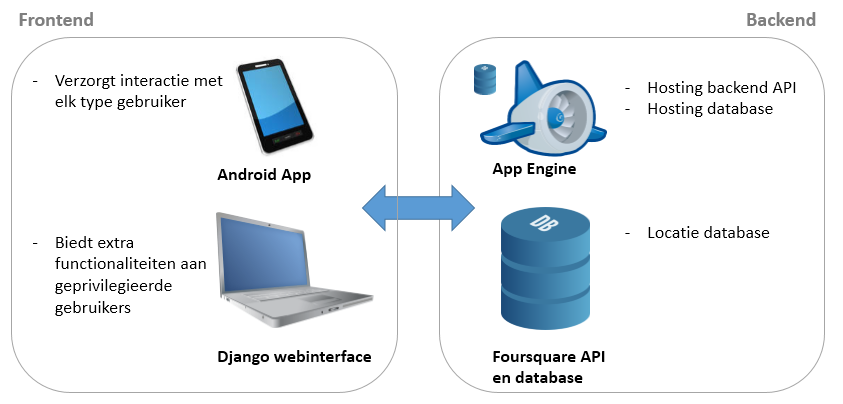
\includegraphics[scale=0.5]{achitectuur}
	\caption{Architectuur bestaat uit twee grote delen, enerzijds de backend en anderzijds de frontend. De backend bestaat uit een combinatie van een App Engine instantie en de Foursquare API. De frontend bestaat uit een Android app en een Django webinterface.}
	\label{fig:algemene structuur}
	
\end{figure}

\section{Backend}

\subsection{Google Cloud Endpoints}
\label{sec: GCE}

Google Cloud Endpoints (GCE) is een uitbreiding van Google App Engine (GAE). GAE is een bekend `Platform as a Service' ontworpen om applicaties uit te voeren op Google's infrastructuur. GCE biedt naast de functionaliteiten beschikbaar in GAE de mogelijkheid om op een relatief eenvoudige manier een backend API te genereren voor applicaties.  Endpoints verzorgt onder andere de communicatie en authenticatie tussen gebruikers en de backend.
Aangezien GCE nog steeds gehost wordt door een Googles App Engine instantie blijven alle andere functionaliteiten zoals `Datastore' voor dataopslag, `Google Cloud Messaging' voor notificaties en `Cron Jobs' voor periodieke taken beschikbaar.

Het voornaamste voordeel van het werken met GAE is dat er tijdens ontwikkelfase geen rekening hoeft gehouden te worden met het  beheer en de administratie van de backend infrastructuur. Een probleem zoals schaalbaarheid wordt via dynamische rekenkrachtallocatie opgelost. Daarnaast is de backend van Triump ook altijd bereikbaar aangezien GAE een hoge graad van permanentie van zijn servers verzekert. Desalniettemin brengt het gebruik van GAE ook enkele nadelen met zich mee. De voornaamste zijn de restricties op het aantal lees- en schrijfoperaties per dag, de sterk variërende tijdsduur van lees- en schrijfoperaties en de afhankelijkheid van een externe organisatie. De restricties op het aantal operaties zijn enkel aanwezig bij gratis gebruik van GAE en kunnen geremediëerd worden door te betalen voor de diensten van GAE.
Aangezien elke nieuwe ontwikkelaar \$ 300 in GAE krediet krijgt, kon dit probleem tijdens de ontwikkelfase opgelost worden door het aantal operaties per dag van 50.000 naar 1.000.000 te verhogen. Een groot aantal operaties is vereist omdat elke atomaire  leesoperatie/schrijfoperatie wordt meegerekend. Indien bijvoorbeeld een groep met zijn leden opgehaald wordt uit de database, moet voor elk lid een leesoperatie gebeuren. Hierdoor neemt het aantal leesoperaties/schrijfoperaties bij het uitvoeren van enkele complexe operaties zeer snel toe. De tijdsduur van operaties op de GAE kan beperkt worden door te investeren in snellere apparatuur (met GAE krediet). Hiervoor werd tijdens de ontwikkeling niet gekozen.

\subsubsection{Datastore~\cite{Google_Datastore}}

Triump maakt gebruik van App Engine Datastore als backend databank. GAE Datastore verschilt van traditionele relationele databases door zijn specifieke architectuur. De database is namelijk zo ontworpen dat deze automatisch meeschaalt met toenemende hoeveelheid opgeslagen data. Een tweede verschil is dat de GAE Datastore schemaloos is. Dit houdt in dat er geen restricties worden opgelegd op de data. Voorbeelden van dergelijke restricties zijn: een attribuut is van een bepaald type is, een vreemde sleutel moet bestaan, een primaire sleutel moet uniek zijn,\ldots. Bijgevolg ligt de verantwoordelijkheid van de integriteit van de databank volledig bij de ontwikkelaar.

\subsubsection{Google Cloud Messaging~\cite{Google_Cloud_Messaging}}

Google Cloud Messaging (GCM) voor Android is een dienst die het mogelijk maakt data (tot 4kB) te versturen van backend servers naar Android applicaties onder de vorm van boodschappen. De GCM servers staan in voor de connectie naar het mobiele toestel en een correcte aflevering van de berichten. De ontvangen boodschappen kunnen na aflevering eenvoudig omgevormd worden tot een notificatie. GCM wordt daarom gebruikt als basistechnologie voor het notificatiesysteem in Triump.

\subsubsection{Cron jobs~\cite{Google_Cron_Jobs}}

Een van de functionaliteiten die Google App Engine aanbiedt is de App Engine Cron Service. Deze service laat gebruikers toe bepaalde taken (cron jobs/chronical jobs) op regelmatige tijdstippen uit te laten voeren op de backend. Bovendien blijft de GAE instantie actief op de servers, door het gebruik van Cron Jobs, waardoor deze niet steeds opnieuw opgestart dient te worden bij lange timeouts tussen requests. Dit probleem wordt uitgebreid besproken in sectie \ref{tijdsduur}.


\subsection{Foursquare API}
\label{Foursquare API}
Triump is een locatie-gebaseerde applicatie. In de applicatie worden locaties verkregen via de Foursquare API en locatiedatabase \cite{FS_API_website}. Naast locatiegegevens kan er ook informatie van gebruikers zoals namen, geboortedata en profielfoto's opgevraagd worden.
Het grote voordeel van de Foursquare API is dat locatiedata niet door de gebruikers zelf moet gegeneerd worden. Bovendien komt Triump, door deel van de functionaliteit van Swarm en Foursquare over te nemen, bij de gebruikers als vertrouwd over; een deel van de bestaande userbase kan overgenomen worden. 
Het gebruikte mechanisme in de Foursquare API is zeer vanzelfsprekend. Alle gegevens, opgeslaan in de database, zijn benaderbaar via een RESTful (Representational State Transfer) URL. De frontend applicatie dient een connectie over HTTPS te starten met een Foursquare API Endpoint via de gewenste URL. Vervolgens zal de API Endpoint de gevraagde informatie in JSON (Javascript Object Notation) formaat terugzenden. JSON is een gestandaardiseerd gegevensformaat.
Het werken met de API brengt echter wel enkele nadelen met zich mee.
Allereerst wordt Triump hierdoor opnieuw afhankelijk van een externe organisatie (naast Google). Indien Foursquare beslist zijn open database te sluiten moet het ontwerp van Triump volledig herzien worden. Daarnaast wordt van commerciële applicaties verwacht dat ze reclame maken voor Foursquare door bijvoorbeeld het Foursquare logo op te nemen in de layout.  Een tweede nadeel is dat de dataopslag verdeeld wordt over twee databases. Enerzijds de Google Cloud Datastore waar de data over groepen en checkins worden bijgehouden en anderzijds de Foursquare Datastore waar de locatie en gebruikergegevens zijn opgeslagen. Een laatste nadeel is dat locaties verplicht geregistreerd moeten zijn bij Foursquare teneinde zichtbaar te zijn op Triump. 
Indien locaties intern zouden aangemaakt en opgeslagen worden, zijn de eerste twee nadelen verholpen. Deze voor de hand liggende oplossing wordt echter niet toegepast aangezien dit zou impliceren dat Triump vanaf nul zijn locatiedatabase zou moeten aanvullen. Hierdoor worden gebruikers ontmoedigd om Triump boven Foursquare te kiezen. Daarnaast propageert Triump een checkin door naar Foursquare waardoor Triump de basisfunctionaliteiten van Foursquare breidt. 
Het laatste probleem wordt opgelost door het voorzien van een webinterface. Deze interface voorziet de mogelijkheid aan eigenaars om locaties te registreren. Meer uitleg over de website volgt in sectie \ref{Webinterface}.
\section{Frontend}
\subsection{Android applicatie}
\subsubsection{Waarom Android?}

Bij de ontwikkeling van de Triump applicatie is er gekozen voor Android als mobiel platform boven iOS of Windows Phone. Android heeft als voordeel dat het een groot marktaandeel heeft (76.6\% van de smartphones wereldwijd draait op Android \cite{marketshare}) en er dus een groot publiek bereikt kan worden met de applicatie. Dit maakt dat Android als eerste platform de beste keuze is. De ontwikkeltools voor iOS en Windows Phone zijn bovendien niet cross-platform. Om apps te ontwikkelen voor iOS dient men over XCode te beschikken (enkel beschikbaar op Mac OS X) en om Windows Phone applicaties te ontwikkelen maakt men gebruik van Visual Studio (enkel beschikbaar op Windows). Vermits het team bestaat uit 1 Windows, 1 Linux en 2 Mac gebruikers, was het noodzakelijk om een cross-platform ontwikkelomgeving te hebben.
Momenteel wordt het proof of concept dus ontwikkeld in Android, en ondersteuning voor andere systemen volgt later.
\subsubsection{Ontwikkelomgeving: Android Studio}
% vergelijking vs Eclipse
Vroeger was Eclipse de standaard ontwikkelomgeving (IDE) voor Android. Hierbij werd de standaard Eclipse installatie uitgebreid met de Android Developer Toolkit (ADT) plugin om Eclipse beter geschikt te maken voor Android Development. Op 16 mei 2013 stelde Google de nieuwste IDE voor Android voor genaamd Android Studio. Deze IDE is gebaseerd op IntelliJ IDEA en biedt veel verbeteringen ten opzichte van Eclipse. 
De voordelen van Android Studio zijn legio: betere code generatie en auto-complete dan Eclipse, zeer goede integratie met de Android SDK en live previews in de layout builder. 

%\begin{figure}[H]
%	\centering
%	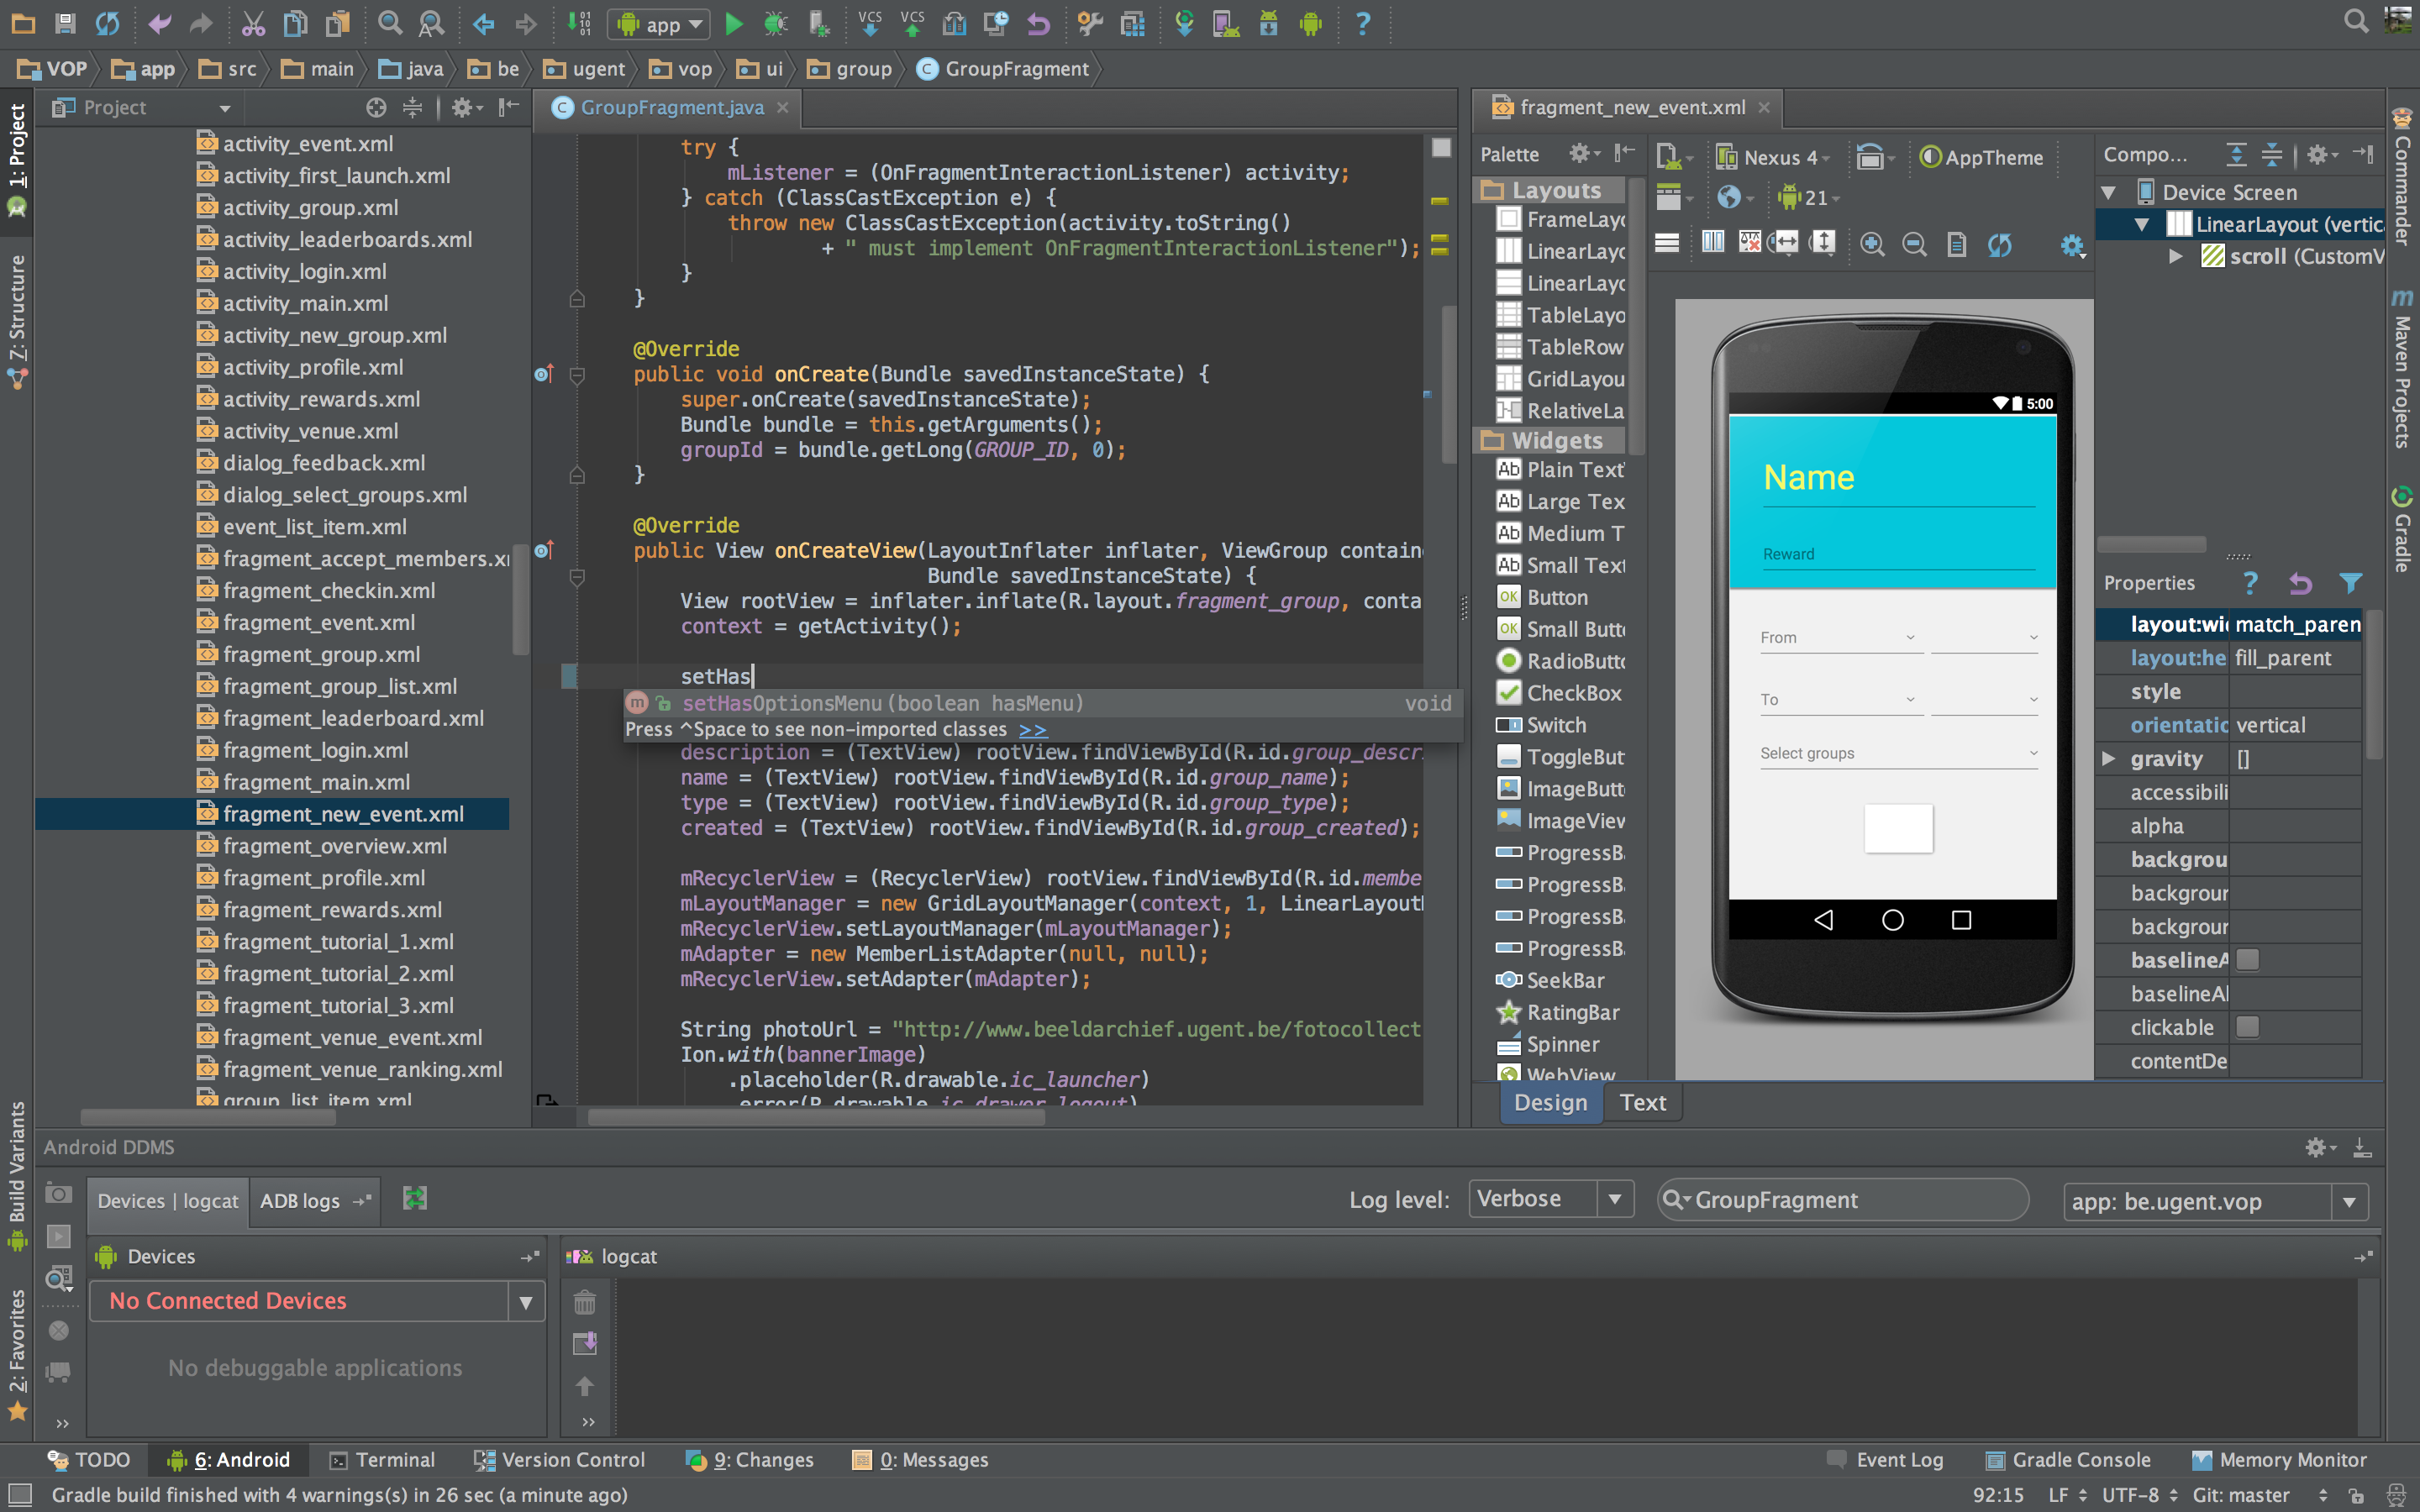
\includegraphics[width=\linewidth]{android_studio}
%	\caption{Een typische workflow in Android Studio}
%	\label{fig:Android Studio Workflow}
%\end{figure}

\subsection{Webinterface}
\label{Webinterface}
\subsubsection{Doel}
Voor een aantal taken is een smartphone niet helemaal geschikt. Zulke taken zijn o.a. het beheren van groepen en het aanmaken van officiele evenementen.
Deze taken gebeuren met bepaalde regelmaat en zijn gemakkelijker op een groter scherm uit te voeren. Specifieke gebruikers, zoals uitbaters van locaties die een promotie willen opzetten als online marketing strategie, zullen deze taken willen uitvoeren via een overzichtelijke webinterface. Daarom is Triump uitgebreid met een webinterface die bereikbaar is via de publieke website van Triump\cite{triumpsite}.
Deze site zal tevens dienst doen als infopunt voor huidige en toekomstige gebruikers. 

Op de site staat informatie over het doel van Triump, en wordt er een link voorzien zodat toekomstige gebruikers de applicatie kunnen downloaden.
Op de website kunnen gebruikers net als in de Android-applicatie inloggen met Foursquare. Het is de bedoeling dat het registreren van een Foursquare-locatie steeds via de website gebeurd, net als het aanmaken van promoties door een eigenaar van een registreerde locatie. Het opleggen van registratie van een locatie door de eigenaar moet ervoor zorgen dat er geen valse promoties worden opgezet. Zonder registratie zou immers iemand een promotie kunnen aanmaken voor een bepaalde locatie zonder dat deze ook daadwerkelijk wordt gegeven.

\subsubsection{Django-framework}
Bij het maken van een website zijn er verschillende keuzes.
Eerst en vooral is er de keuze of er gebruik wordt gemaakt van een bestaand framework, zoals Ruby on Rails, ASP.NET en Django, of dat men zelf de nodige functionaliteit implementeert met bijvoorbeeld PHP.
Bestaande frameworks bieden ruim voldoende functionaliteit aan om de Triump website te verwezenlijken. De frameworks zijn bovendien reeds geoptimaliseerd en bevatten o.a. methoden om op een veilige manier aan authenticatie te doen.
Daarnaast moet men nog kiezen om ofwel de site bij een hosting-dienst te plaatsen, ofwel zelf de site te hosten op een eigen pc. Gebruik maken van een bestaande hosting-dienst, is het eenvoudigst. Voor een vast bedrag, per maand of jaar, wordt de website geplaatst op de servers van de hosting-dienst. Deze neemt extra moeilijkheden, zoals het instellen en onderhouden van DNS-servers op zich.

Op de site worden gebruikers aangemaakt waarbij bepaalde informatie wordt opgeslaan, zoals hun Foursquare-identiteit, zodat de gebruiker maar 1 keer met Foursquare moet inloggen. Dit gebeurt aan de hand van een DBMS-systeem. \\

Als framework voor de webinterface werd gekozen voor Django, een framework geschreven in Python. Django maakt het mogelijk om op relatief korte tijd toch een dynamische website te bouwen.
Een voordeel van het werken met Django is dat er hosting-diensten bestaan die zich specialiseren in het hosten van Django-projecten. Wij kozen voor zo een dienst\cite{djangoeurope}.
Bij deze dienst was er de mogelijkheid te kiezen uit verschillende databasemanagment systemen. Er werd gekozen voor PostgreSQL: een open source DBMS waar reeds mee gewerkt werd tijdens het vak `Databanken'.
Communicatie tussen de backend en de website verloopt via Javascript. Google biedt namelijk een API aan die het mogelijk maakt om Google Endpoints via Javascript aan te spreken. Zo wordt gemakkelijk een van de functies uit de backend opgeroepen en kan het resultaat, dat in JSON wordt ontvangen, ook vlot worden verwerkt met behulp van Javascript. Deze keuze brengt wel nadelen met zich mee. Aan de basis van deze nadelen ligt het feit dat Javascript op de computer van de gebruiker wordt uitgevoerd, en niet op de server die de website host. Op sommige computers is Javascript namelijk niet is geïnstalleerd. Het `client-side' uitvoeren van code brengt nog een ander nadeel met zich mee: het vormt namelijk een zwak punt in de verdediging tegen aanvallen van buitenaf. Een alternatief is het gebruiken van een python-module op de webserver die communicatie met Google Endpoints mogelijk maakt. Deze code wordt `server-side' uitgevoerd. De backend is echter in Java geprogrammeerd, hetgeen gebruik van de python-module bemoeilijkte.

\chapter{Ontwerp}
Figuur \ref{fig:algemene structuur backend} geeft een abstract overzicht van de verschillende onderdelen van de backend en van de interacties tussen backend en frontend. De pijlen tussen de verschillende onderdelen in de figuur worden in de volgende secties verklaard.

\begin{figure}[H]
	\centering
	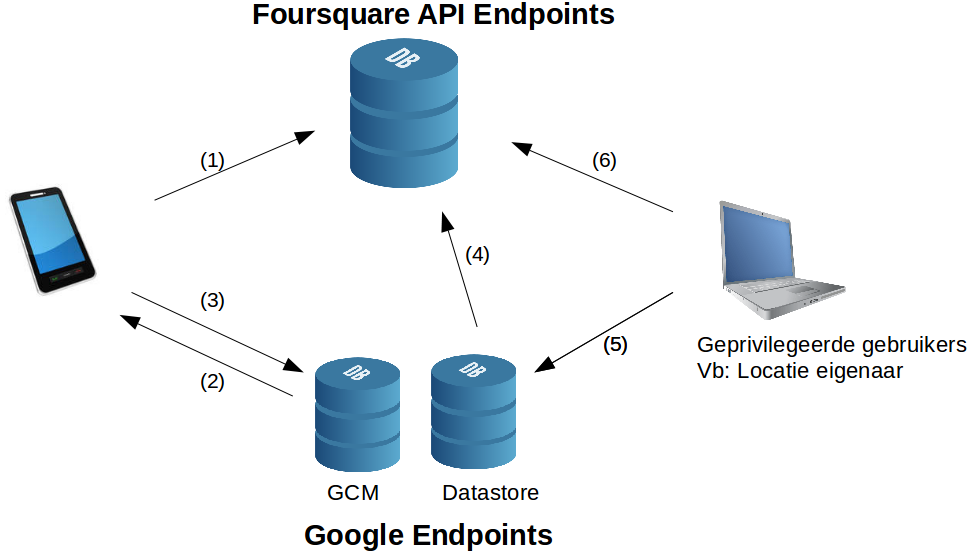
\includegraphics[scale=0.3]{backend_algemene_structuur}
	\caption{Overzicht interactie tussen de frontend en de backend (pijlen worden in onderstaande secties verklaard).}
	\label{fig:algemene structuur backend}
	
\end{figure}
\section{Backend}
\subsection{Database}
Zoals reeds aangegeven word de backend database gehost op een GAE instantie. De GAE Datastore is schemaloos wat impliceert dat er geen enkele restrictie met betrekking tot de opbouw van entiteiten wordt opgelegd. Toch is er gekozen voor de database te ontwerpen volgens de principes van een relationele databank. Het behoud van de integriteit van de data ligt nu wel volledig bij de ontwikkelaars. 

Figuur \ref{fig:Backend ER} toont een ER diagram van de backend database.  De belangrijkste entiteiten van deze database zijn User, Event, Venue, Group en Checkin. In de volgende paragraaf wordt de structuur van de database besproken. 

Een user entiteit wordt aangemaakt wanneer een gebruiker zich voor het eerst authenticeert bij de backend. Het ID van een gebruiker in de Triump database is identiek aan het ID van een gebruiker in de Foursquare database. Aangezien er in de Foursquare databank `strings' worden gebruikt als primaire sleutel hebben ook User-entiteiten `string' ID's.  Informatie zoals voornaam, achternaam en e-mailadres van een gebruiker wordt bekomen via een request naar de Foursquare API. In sectie \ref{Foursquare API} komt de werking van de Foursquare API aan bod. Pijl (4) van figuur \ref{fig:algemene structuur backend} geeft de afhankelijkheid tussen Triumps database en de Foursquare database weer.

Venue-entiteiten worden aangemaakt wanneer een gebruiker voor het eerst incheckt op een nieuwe locatie. Opnieuw is de ID van een venue entiteit identiek aan het ID van de entiteit binnen Foursquare. Een datum en tijdstip van de eerste checkin wordt bijgehouden. Deze informatie kan gebruikt worden om statistieken van locaties te genereren. Een locatie of venue heeft een `verified' attribuut indien een gebruiker zich via de webinterface (zie sectie \ref{Webinterface} voor meer informatie over het doel en de werking van de webinterface) verifieert. Een geverifieerde gebruiker (meestal een locatie-eigenaar) in combinatie met een geverifieerde locatie kan een evenement organiseren waaraan elke groep, indien zij voldoen aan de opgelegde participatievoorwaarden, kan deelnemen. Aan de winnaar van het evenement kan dan een promotie toegekend worden.

Zoals reeds aangehaald zijn er enerzijds `officiële' evenementen waarbij promoties verkregen kunnen worden. Anderzijds zijn er ook evenementen die gebruikers voor hun vrienden organiseren. Deze evenementen kunnen aangemaakt worden door elke gebruiker. Aangezien deze gewone evenementen niet automatisch zichtbaar zijn moet de organisator groepen, waartoe hij of zij zelf behoort, uitnodigen. 
Deze twee types evenementen worden beiden opgeslagen in Event-entiteiten. Het `verified' veld geeft aan of een Event entiteit een officieel of gewoon Event is. De attributen `minParticipants' en `maxParticipants' hebben enkel een geldige waarde voor evenementen met promoties. De organisator hiervan kan beslissen een verschillende promotie te lanceren voor groepen met een bepaalde grootte of type. De entiteit GroupEvent wordt gebruikt om bij te houden welke groepen er zijn uitgenodigd op een gewoon evenement.

Een Checkin entiteit wordt aangemaakt iedere keer een gebruiker incheckt op een locatie. Het `points' veld geeft aan hoeveel punten een checkin waard is. De attributen tijdstip en groep worden bijgehouden om later te bepalen welke groep een event heeft gewonnen en om de ranglijsten op te stellen. (Meer informatie over deze berekeningen volgt in sectie \ref{backend API}: Backend API.)

Elke gebruiker van Triump is in staat zijn eigen groepen aan te maken. De maker van een groep is ook de administrator ervan. Opnieuw kan het `type' attribuut gebruikt worden om statistieken te generen van de beste studentvereniging of meest actieve vriendengroep. `numMembers' is afgeleide data aangezien de waarde kan berekend worden uit het aantal entiteiten in de UserGroup tabel. Toch wordt `numMembers' bijgehouden in Group-entiteiten aangezien dit een waarde is die vaak gebruikt wordt. Voordelen hiervan zijn een verbetering van de performantie en een vermindering van het aantal leesoperaties. Een nadeel is de mogelijkheid tot het optreden van anomalieën.

UserGroup-entiteiten koppelen een gebruiker met een groep. Een entiteit wordt aangemaakt wanneer een gebruiker een aanvraag doet om tot een groep te behoren. Het `accepted' attribuut wordt bij de aanmaak op 0 geplaatst tot de administrator toestemming geeft aan de gebruiker om lid te worden van de groep. Indien de administrator het lidschapverzoek weigert, wordt de entiteit verwijderd.

Tot slot wordt in UserEvent-entiteiten bijgehouden welke gebruikers een evenementen gewonnen hebben en bijgevolg van de promotie gebruik mogen maken. Het `received' attribuut geeft aan indien een gebruiker zijn promotie reeds heeft gebruikt.

Het ontwerp van de backend database focust enerzijds op functionaliteit (alle functies die Triump wil aanbieden moeten namelijk mogelijk zijn met de backend) en anderzijds op het bijhouden van informatie voor statistieken. Indien Triump gebruikt zal worden als online marketing tool, is het belangrijk om statistieken te genereren over het gebruik van de toepassing om zo locatie-eigenaars aan te kunnen geven hoe ze Triump het best gebruiken. Bovendien zijn statistieken ook voor andere gebruikers interessant.

Figuur \ref{fig:Backend ER 2} toont het overige deel van de backend database. Wanneer een gebruiker zich voor het eerst authenticeert met de backend wordt er een SessionToken gekoppeld met de gebruiker. Deze token wordt meegegeven als parameter met iedere API call om de een gebruiker te authenticeren. De GCM tabel van de backend database houdt voor iedere gebruiker een gcmId bij. Deze ID wordt gebruikt voor de Google Cloud Messaging dienst.

\begin{figure}[H]
	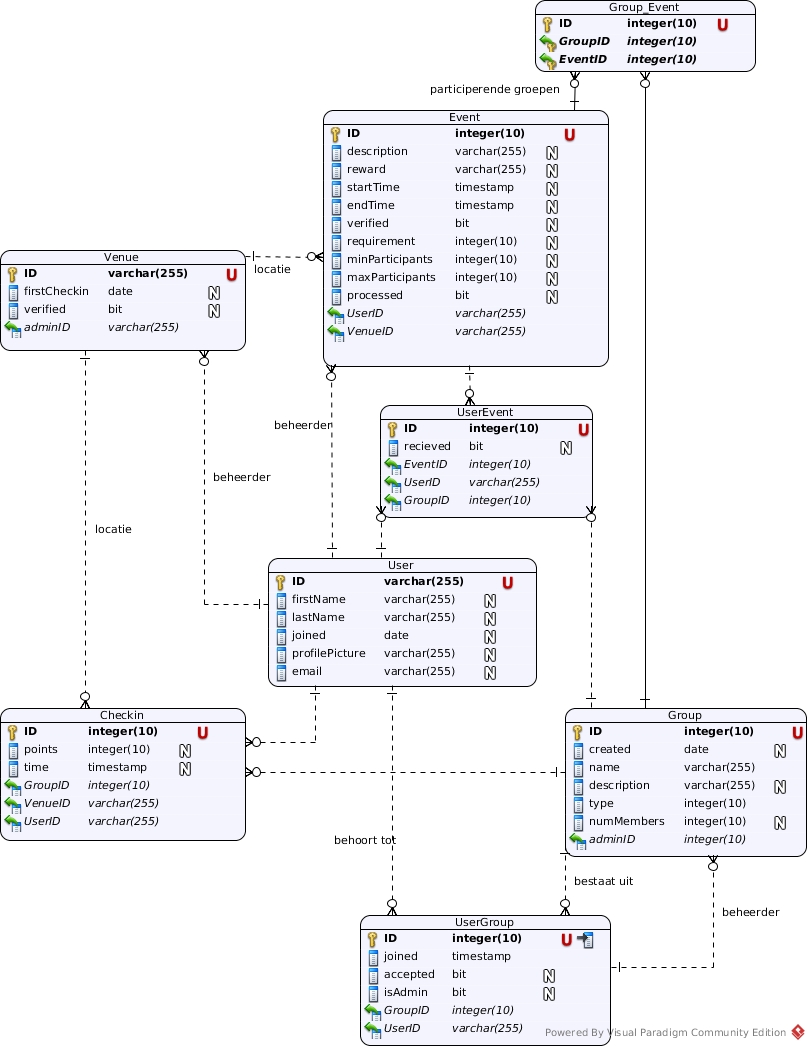
\includegraphics[scale=0.43]{backend_EER}
	\caption{Entity Relation diagram van de backend database. \textsc{opmerking}: Het Boolean type wordt weergegeven als Bit aangezien de Community Edition van Visual Paradigm, Booleans niet ondersteunt. }
	\label{fig:Backend ER}
\end{figure}


\begin{figure}[H]
	\centering
	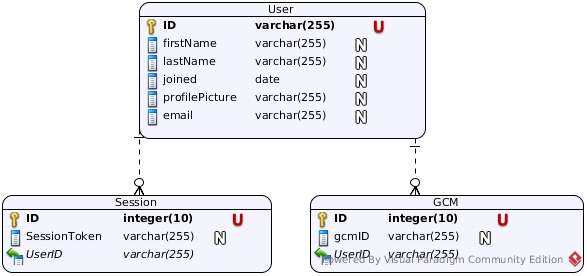
\includegraphics[scale=0.35]{backend_EER_deel2}
	\caption{Entity Relation diagram van het administratieve deel van de backend database}
	\label{fig:Backend ER 2}
\end{figure}
\subsection{Google Cloud Messaging}
GCM wordt in Triump gebruikt als basis van het notificatie systeem. In de huidige implementatie ontvangt een gebruiker een notificatie indien hij/zij een event heeft gewonnen of indien er om feedback wordt gevraagd. 
Pijl (2) van figuur \ref{fig:algemene structuur backend} geeft aan dat er via GCM, vanop de backend servers, berichten worden gepusht naar de gebruikers.

\subsection{Cron jobs}
In het geval van de backend van Triump is het noodzakelijk om beloningen (rewards) na het aflopen van evenementen voor gebruikers te laten genereren. Hiervoor wordt gebruik gemaakt van een cron job, die geconfigureerd wordt in een Java servlet. 

\subsection{Backend API}
\label{backend API}
De backend API bestaat uit een reeks methodes die kunnen opgeroepen worden vanop het mobiele toestel of vanop de webinterface. Dit is weergegeven met pijlen (3) en (5) op figuur \ref{fig:algemene structuur backend}. Een groot deel van de methodes hebben als doel het ophalen van gegevens uit de database, deze gegevens te mappen op een klasse om vervolgens een object terug te geven als resultaat. Deze objecten worden vervolgens gemanipuleerd in de Android toepassing of de webinterface. Een tweede soort API calls wordt gebruikt om entiteiten van de tabellen Group, Event, UserGroup en UserEvent aan te maken of te wijzigen. Een voorbeeld van zo een methode is generateRewards(). De methode generateRewards() wordt vanuit een Cron Job (zie sectie \ref{sec: GCE} Cron jobs) ieder kwartier opgeroepen. Prinicipieel werkt de functie als volgt:
\begin{enumerate}
	\item Controleer of er het afgelopen kwartier een event is beëindigd.
	\item Bereken voor elk beëndigd event welke groepen gewonnen zijn a.d.h.v. de tijdstippen van de Checkin entiteiten. Hierbij wordt er rekening gehouden met participatievoorwaarden zoals het minimaal en maximaal aantal leden van een groep.
	\item De leden van een winnende groep worden geplaatst in de UserEvent tabel.
	\item Via het notificatiesysteem (zie sectie \ref{sec: GCE} Google Cloud Messaging) worden de winnende gebruikers verwittigd.
\end{enumerate}
Voor elke functie in de backend is een algoritme uitgewerkt waarbij steeds rekening gehouden wordt met efficiëntie (wegens het beperkt aantal atomaire operaties aangeboden door GCE, zie \ref{sec: GCE})
Tot slot bevat de backend API nog methodes die gebruikers registeren, gebruikers authenticeren en communiceren met de GCM diensten. 

\subsection{Foursquare API}
Het mobiele toestel zal rechtstreeks requests sturen naar de Foursquare API om bijvoorbeeld een lijst te krijgen van dichtbijzijnde locaties of om informatie van een locatie op te vragen. Het gebruik van de API wordt getoond in figuur \ref{fig:algemene structuur backend} via pijl (1).


\section{Frontend}
\subsection{Android applicatie}

\subsubsection{Ontwerpkeuzes}
Tijdens de ontwikkeling van Triump is er voor gekozen om te werken met de nieuwste technologieën voor Android. Dat houdt in dat Triump ontwikkeld is met als doel volledig compatibel te zijn met de laatste versie van Android: 5.1 Lollipop. Triump is daarnaast wel nog steeds compatibel met alle Android versies vanaf 4.1 Jelly Bean. Hierdoor bereikt de applicatie 87,5\% van alle Android toestellen \cite{market_share}. 
Android development gebeurt in Java, maar er zijn enkele Android-specifieke ontwerppatronen waarvan er gebruik gemaakt wordt. Onder andere voor het asynchroon laden van informatie, het opslaan van data en het opbouwen van efficiënte UI lijsten zijn er speciale ontwerppatronen in Android. Deze zullen in de volgende secties verder uitgelegd worden.

\subsubsection{Design}
Triump is ontwikkeld volgens de design richtlijnen van de laatste versie, Android Lollipop. Dit houdt in dat er gebruik gemaakt wordt van de Material Design Guidelines \cite{Material_Design}. Door de Material Design Guidelines te volgen is het makkelijker om een consistent look-and-feel te verkrijgen in de app die volledig in lijn ligt met de rest van het huidige Android ecosysteem.
Om de correcte implementatie van Material Design te garanderen, is er gebruik gemaakt van enkele externe bibliotheken. Deze bibliotheken bieden extra functionaliteit ten opzichte van de standaard Android API waardoor het makkelijker is het correcte design te verkrijgen. Deze bibliotheken zijn steeds backwards compatible met eerdere versies van Android. Hierdoor wordt er een uniforme look verkregen op alle versies die de app ondersteunt.
De gebruikt bibliotheken om Material Design te implementeren zijn:
\begin{description}
	\item[Material Design Library \cite{navasmdc}] Een bibliotheek die verschillende UI componenten bevat die voldoen aan de Material Design Guidelines zoals de Flat Buttons, Progress Bar Indicators en Switches.
	\item[FloatingActionButton \cite{floatingactionbutton}] Een bibliotheek die de Floating Action Button van de Material Design Specification implementeert en toelaat om die toe te voegen aan een RecyclerView (zie verder).
	\item[MaterialEditText \cite{materialedittext}] Een bibliotheek die een consistent implementatie biedt voor tekstvelden in formulieren. De bibliotheek voorziet verschillende functies voor de tekstvelden zoals maximum lengte, hints, iconen en aangepaste kleuren.
\end{description}

\subsubsection{RecyclerView}
Sinds Android 5.0 is er een nieuwe manier geïntroduceerd om lijsten weer te geven in de UI van de applicatie. Onze applicatie maakt veelvuldig gebruik van lijsten (groepen, locaties, evenementen,...) en bijgevolg wordt gestreefd om van de laatste standaard hieromtrent gebruik te maken. Deze nieuwe widget (zo heten de UI componenten in Android) is de RecyclerView. De RecyclerView vervangt de oudere ListView widget.
De ListView en RecyclerView geven beiden een lijst weer van data. Beide widgets worden aangestuurd door een zogenaamde DataAdapter. Die Adapter is een speciale klasse die de widgets oproepen om de rijen van de lijsten te vullen met data. Daarvoor moet de Adapter bepaalde methoden implementeren die dan door de ListView / RecyclerView opgeroepen worden. Bij zowel ListView als RecyclerView is 1 van die methodes verantwoordelijk voor het vullen van de View van 1 rij met de correcte data.
Voor elke rij in de lijst is de layout vastgelegd in een XML bestand. Aan de hand van dit XML bestand wordt dan voor elke rij een View object aangemaakt dat de correcte layout bevat. Op dat moment is het View object voor die rij nog niet gevuld met de correcte data. Daarvoor wordt bij de Adapter een methode opgeroepen om die View te vullen met de correcte data.
Het is in deze stap dat RecyclerView en ListView fundamenteel verschillen. In het geval van een ListView zal de Adapter voor elke rij verschillende findViewById operaties moeten uitvoeren. Deze findViewById operaties zijn echter zeer cpu-intensief. Hierdoor is scrollen in traditionele ListViews niet zo vloeiend.
RecyclerView maakt het grootste deel van de findViewById operaties overbodig door standaard gebruik te maken het ViewHolder patroon.
Concreet leidt het nastreven van de laatste Android ontwerppatronen, zoals de RecyclerView, tot een efficiëntere applicatie.

\subsubsection{Loaders}
In Android gebeurt het tekenen en het interageren met de UI, net zoals bij de meeste andere GUI toolkits, op de main thread. Dit betekent dat het inladen van data over het netwerk of van de lokale opslag in een aparte thread moeten plaatsvinden. Is dit niet het geval, dan zal de volledige UI blokkeren want aanleiding kan geven tot een slechte gebruikerservaring.
Om deze redenen bevat Android het concept van Loaders. De bedoeling van Loaders is om data op een asynchrone manier in te laden (dus op een aparte thread) en de resultaten via een callback terug te sturen naar de main UI thread teneinde ze op het scherm weer te geven. 
\newline\newline
De Material Design richtlijnen, Recycler View en Loaders zijn slechts enkele van de methodes die gevolgd werden bij het ontwikkelen van de Android applicatie. Gedurende het volledige ontwerpproces werd op deze manier gestreefd naar een zo efficiënt mogelijke applicatie, ontwikkeld volgens de meest recente standaarden. \cite{successapp}
\subsection{Webinterface}
\begin{figure}[H]
	\centering
	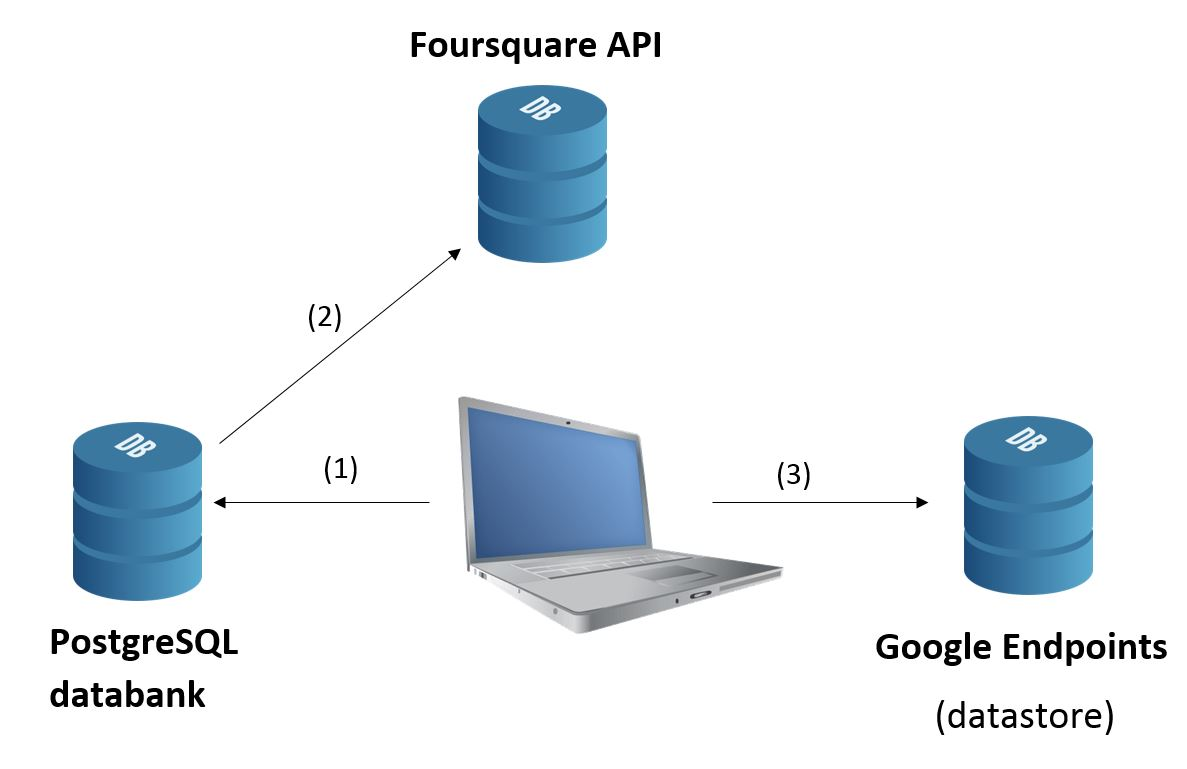
\includegraphics[scale=0.3]{webinterface_structuur}
	\caption{Werking en opbouw webinterface. Zowel de backend datastore als de Foursquare API, via een postgreSQL databank, bieden data aan voor de webinterface. }
	\label{fig:Webinterface}
\end{figure}
De opbouw en werkwijze van de webinterface wordt weergegeven in \ref{fig:Webinterface}. Pijl (1) duidt aan dat de server, die de website host, geconnecteerd is met een PostgreSQL databank. Deze maakt het mogelijk om gebruikers te laten inloggen met een eigen account, waarbij men ook extra data kan opslaan. Er werd reeds aangehaald dat gebruikers ook hier met Foursquare dienen in te loggen, hetgeen gebeurt na registreren. Zoals te zien op de figuur verloopt alle communicatie met de Foursquare API vanop de webserver en niet door de computer van de gebruiker, dit wordt aangeduidt door pijl (2). Deze communicatie omvat het ophalen van locatie- en gebruikergegevens uit de databank van Foursquare.
Pijl (3) geeft weer dat er vanop de computer van de gebruiker wordt gecommuniceerd met de backend (GAE) van Triump. Deze verbinding maakt het mogelijk om vanop de webinterface nieuwe events aan te maken en groepen te beheren.


